\documentclass[11pt,a4paper]{article}

\usepackage{graphicx}
\usepackage{listings}
\usepackage{url}
\title{Accessing GPIO pins of R-Pi}
\author{e-Yantra Team}
\date{\today}

\begin{document}
	\maketitle
	\newpage
	\tableofcontents
	\newpage
	\section{Objective}
	In this tutorial we will learn how to write simple programs to access GPIO pins in an R-Pi. 
	\section{Prerequisites}
	\begin{itemize}
		\item Python programming skills
		\item Basic terminal commands
	\end{itemize}
	\section{Hardware Requirement}
	\begin{enumerate}
		\item Raspberry Pi (I will be using Version 2 Model B)
		\item Power adapter
		\item Connecting wires
		\item LED
		\item Push button
		\item Resistor (330 ohms)
		\item Bread board
	\end{enumerate}
	\section{Software Requirement}
	\begin{enumerate}
		\item PyScripter (version 2.7 or above)
		\item Mobaxterm (for windows users)
	\end{enumerate}
	
	\newpage
	\section{Theory and Description}
	The Raspberry Pi 2 Model B is the second generation Raspberry Pi. Compared to the Raspberry Pi 1 it has:
	\begin{itemize}
	\item A 900MHz quad-core ARM Cortex-A7 CPU
	\item 1GB RAM
	\end{itemize}
	Like the (Pi 1) Model B+, it also has:
	\begin{itemize}
			\item 4 USB ports
			\item 40 GPIO pins
			\item Full HDMI port
			\item Ethernet port
			\item Combined 3.5mm audio jack and composite video
			\item Camera interface (CSI)
			\item Display interface (DSI)
			\item Micro SD card slot
			\item VideoCore IV 3D graphics core
			\item Because it has an ARMv7 processor, it can run the full range of ARM GNU/Linux distributions, including Snappy Ubuntu Core, as well as Microsoft Windows 10. [2]
	\end{itemize}
	
	\textbf{Expansion Header}
	
	The Raspberry Pi 2 Model B board contains a single 40-pin expansion header labelled as 'J8' providing access to 26 GPIO pins.
	(Pins 1, 2, 39 and 40 are also labelled below.)
			\begin{figure}[h!]
				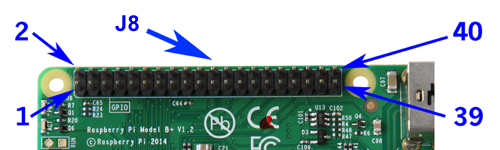
\includegraphics[scale=0.7]{j8h.png}
				\centering
				\caption{[3]}
			\end{figure} 
	
	\newpage
	The diagram below illustrates the pin out diagram of Raspberry Pi 2:
	\begin{figure}[h!]
		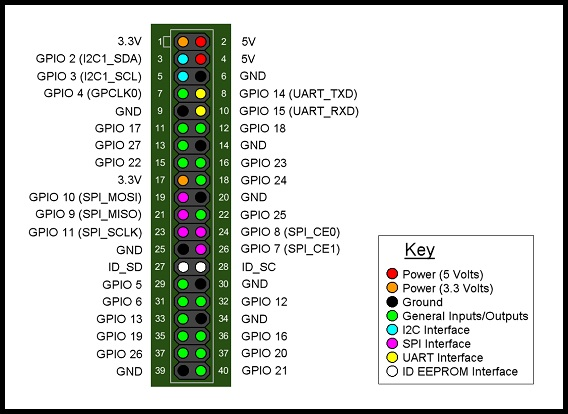
\includegraphics[scale=0.6]{RaspberryPi2_pinout.jpg}
		\centering
		\caption{[4]}
	\end{figure} 
	
	\flushleft
	You must have noticed that the board contains pins named as GPIO (that are used for interfacing input and output devices) and hence in order to refer to the R-Pi pins there exists two modes:
	\begin{enumerate}
		\item \textbf{BCM mode:} Referring the pins with the GPIO number
		\item \textbf{Board mode:} Referring the pins using the IC pin numbers.
	\end{enumerate}
	
	\flushleft
	Raspbian comes preloaded with Python, the official programming language of the Raspberry Pi and IDLE 3, a Python Integrated Development Environment. And hence we can directly program the Pi using Python. Although we can even program the Pi using C language (but i will be using Python language in this tutorial).
	
	\newpage
	\textbf{Different methods to program an R-Pi}
	\newline
	Before we write a code to access GPIO pins of the Pi let's understand the different ways to program Pi.
	\begin{enumerate}
		\item GUI based programming using IDLE3. In order to do so follow these steps:
		\begin{itemize}
			\item First, load up IDLE 3 by double-clicking the icon on your LXDE desktop(either on the monitor or using Mobaxterm as explained in the previous tutorial based on establshing a SSH connection).
			\begin{figure}[h!]
				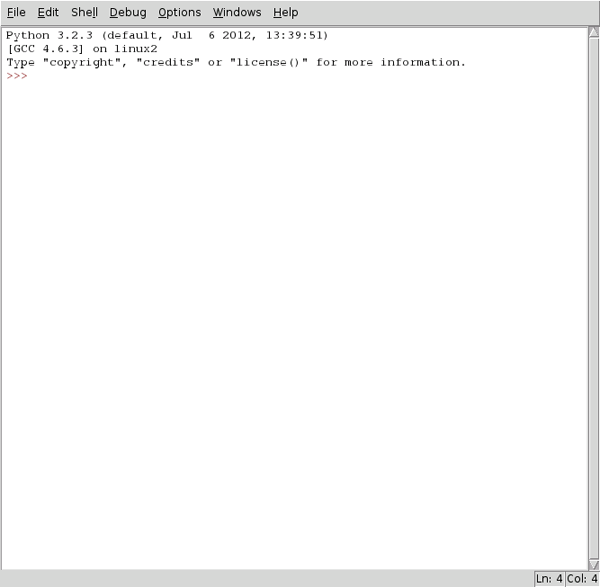
\includegraphics[width=10cm, height=8cm]{idle3.png}
				\centering
				\caption{[1]}
			\end{figure}
			\item Click File,New Window, which will then bring up a new blank window which you can type in.
			\item Now click File,Save As and save your file in the desired folder.
			\item Click Run, and then Run Module or simply press F5.
		\end{itemize}
		\item Terminal based programming:
		\begin{itemize}
			\item Using PyScripter and MobaXterm:
			PyScripter is a free and open-source Python IDE used for programming in Python.In order to download PyScripter use the following link \url{https://code.google.com/p/pyscripter/} (I use version 2.5.3).
			\newline \begin{enumerate}
				\item Open the application. You will see a window like this:
				\begin{figure}[h!]
					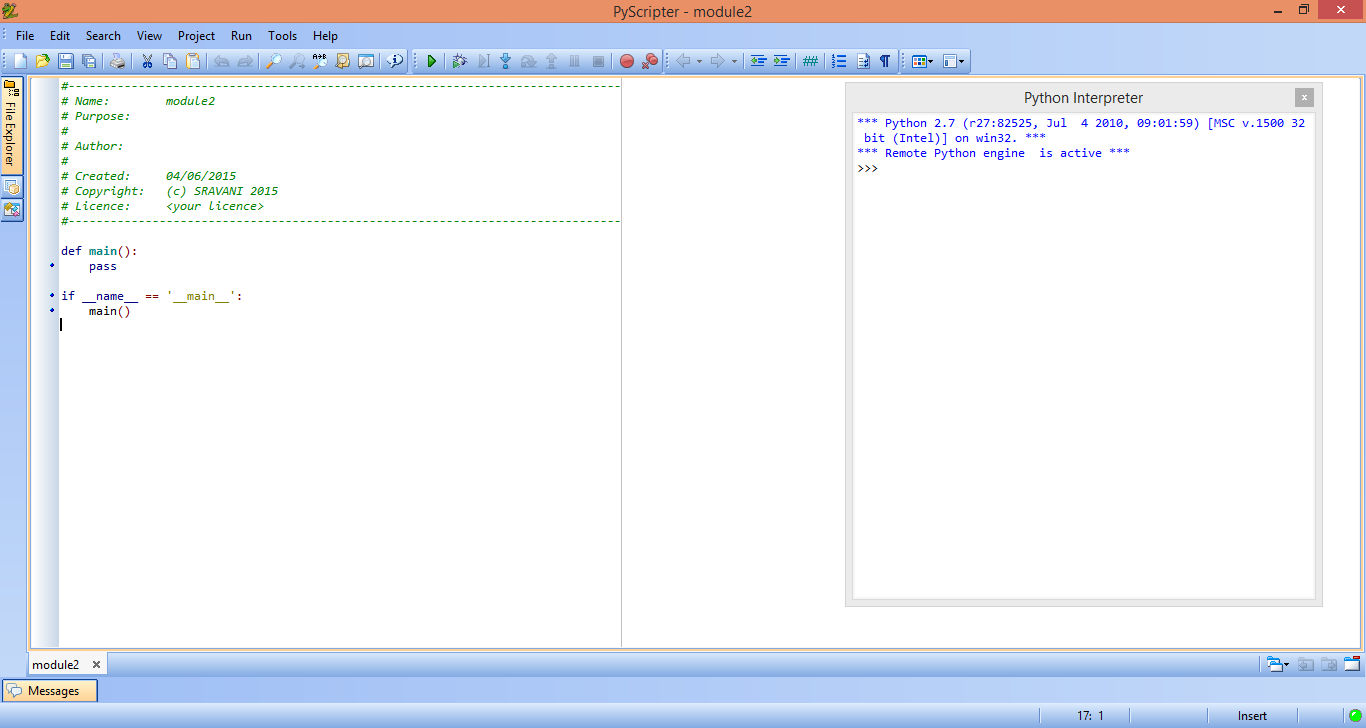
\includegraphics[scale=0.4]{py.png}
					\centering
				\end{figure}
				\item Delete the text already present and type your program. Once you finish typing the program goto File > Save As and save the program.
				\item Now open MobaXterm. On the left side you can see the files in /home/pi/ directory and you also have some small icons on the toolbar. Click on the icon 'Upload to current folder' as shown:
				\begin{figure}[h!]
					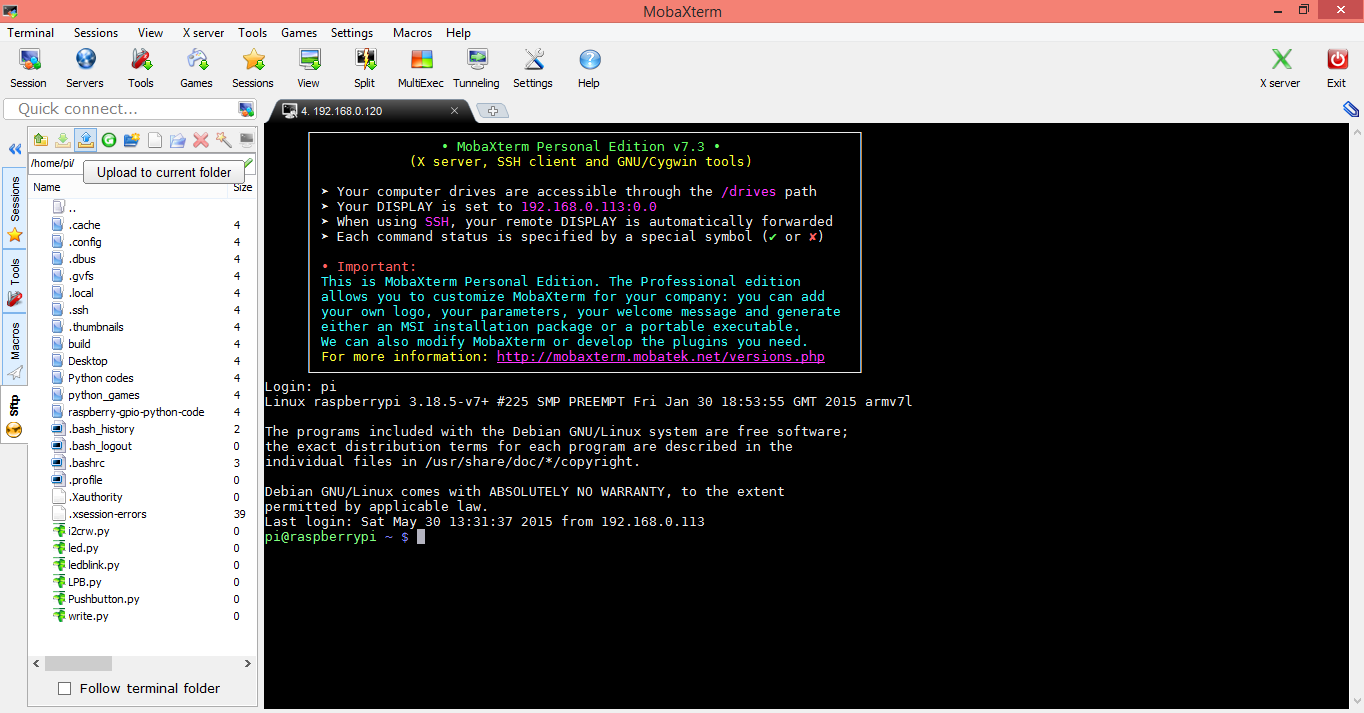
\includegraphics[scale=0.4]{1.png}
					\centering
				\end{figure}
				\newpage
				\item Upload that file wherein you have written your python program.
				Note: You can either upload your files to the home directory i.e. /home/pi/ or else you can create a new directory using the icons on the toolbar as illustrated before and upload your python file over there.
				\item After you have uploaded the code then type the following command on the terminal to execute the code \textit{python filename.py}.
				In case you have uploaded the file to a directory other than home directory then change the path by typing \textit{cd directoryname} and then \textit{sudo python filename.py} (Note: In order to execute files form any directory other than home directory dont forget to use \textit{cd} command before your directory name and textit{sudo python} command before your file name that you want to execute.)
				\begin{figure}[h!]
					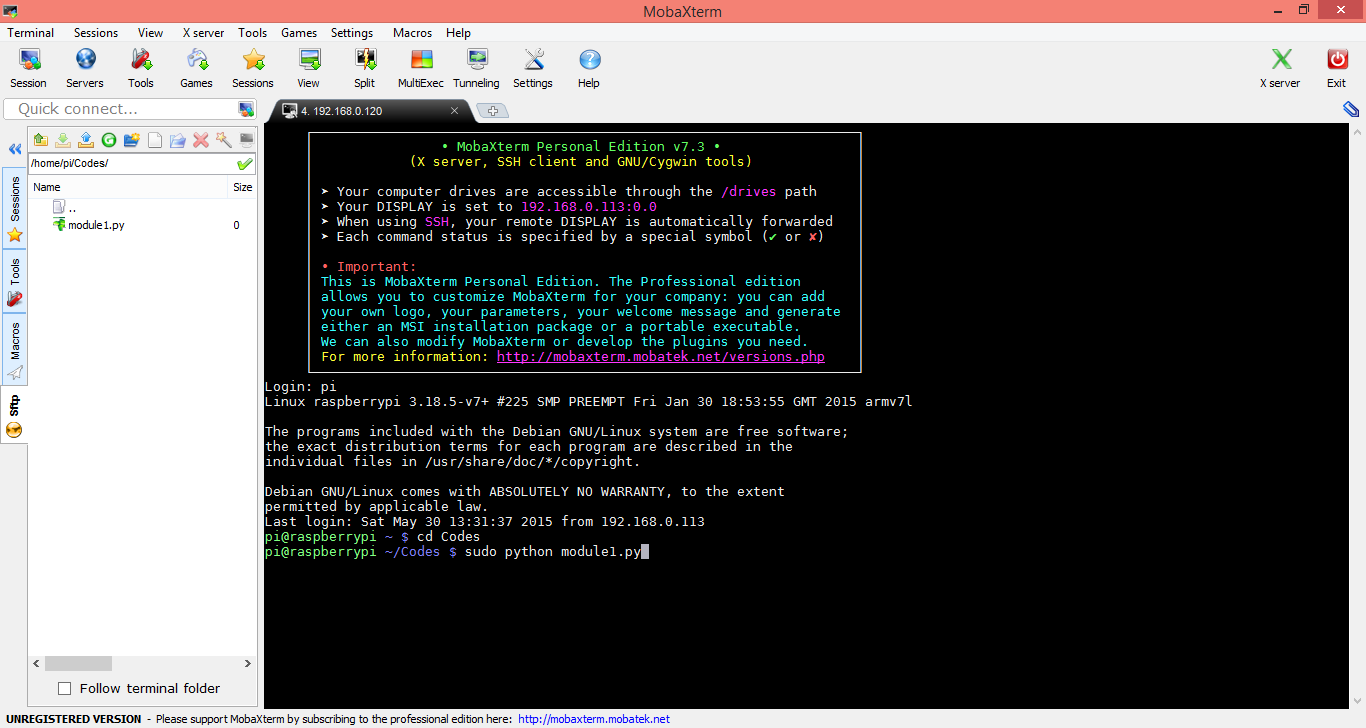
\includegraphics[scale=0.4]{2.png}
					\centering
				\end{figure}
				\end{enumerate}
			\item Using Notepad++ and LXTerminal(or MobaXterm):
			      Notepad++ is a source code and a Windows text editor that is widely used by programmers.(It is more efficient than other text editors because it prompts you with indentation related errors that count in python programming) 
			\begin{enumerate}
				\item Open the application and a create a new file.
				\newpage
				\begin{figure}[h!]
					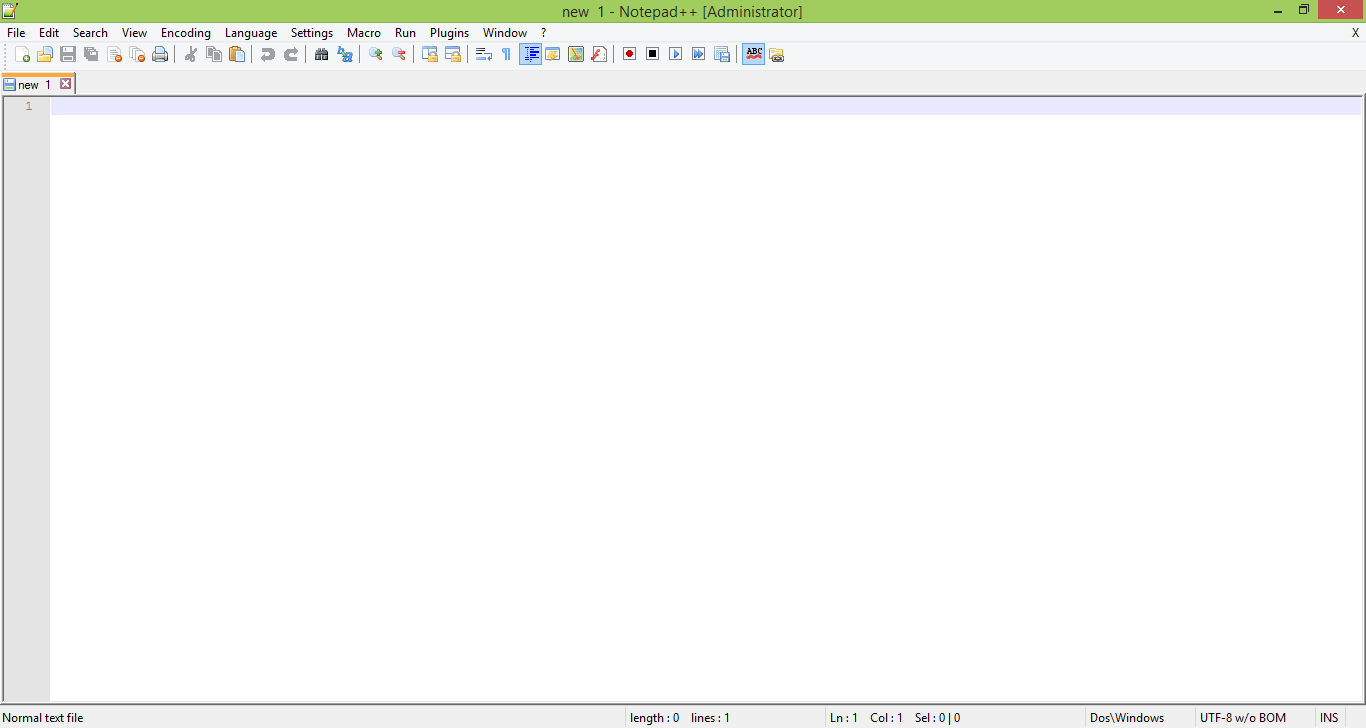
\includegraphics[scale=0.4]{3.png}
					\centering
				\end{figure}
				\item Type your python code and then save it as filename.py 
				\item After that follow the steps(3-5) mentioned in the above method i.e using PScripter and MobaXterm.
			\end{enumerate}
			\item Using MobaXterm(for remote operation) or LXTerminal:
			In this method we can create a python file on the terminal window in the following way:
			\begin{enumerate}
				\item Open the MobaXterm or LXTerminal.
				\item Type the command \textit{touch filename.py} to create a file in a directory say home directory
				\item Once the file is created in order to edit it type the command \textit{nano filename.py}
				\newpage
				\begin{figure}[h!]
					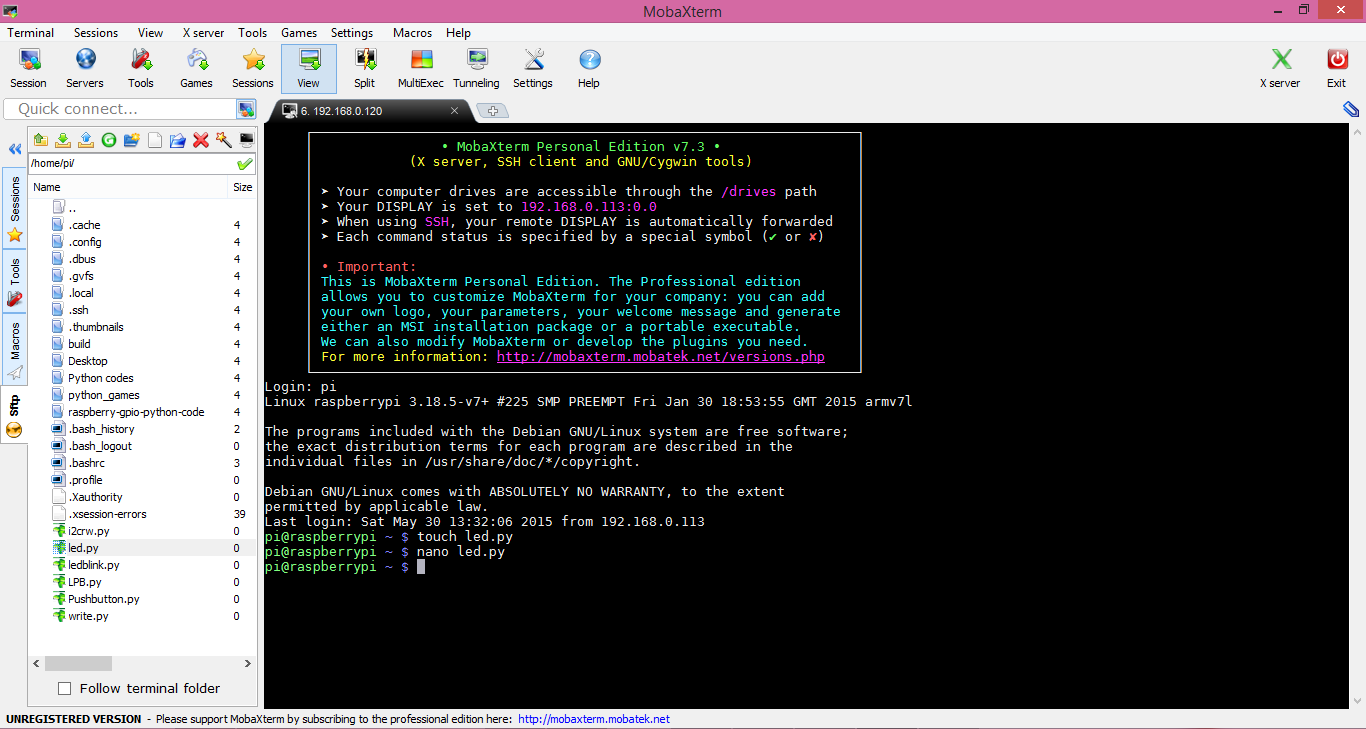
\includegraphics[scale=0.4]{4.png}
					\centering
				\end{figure}
				\item A blank file opens as shown 
				\begin{figure}[h!]
					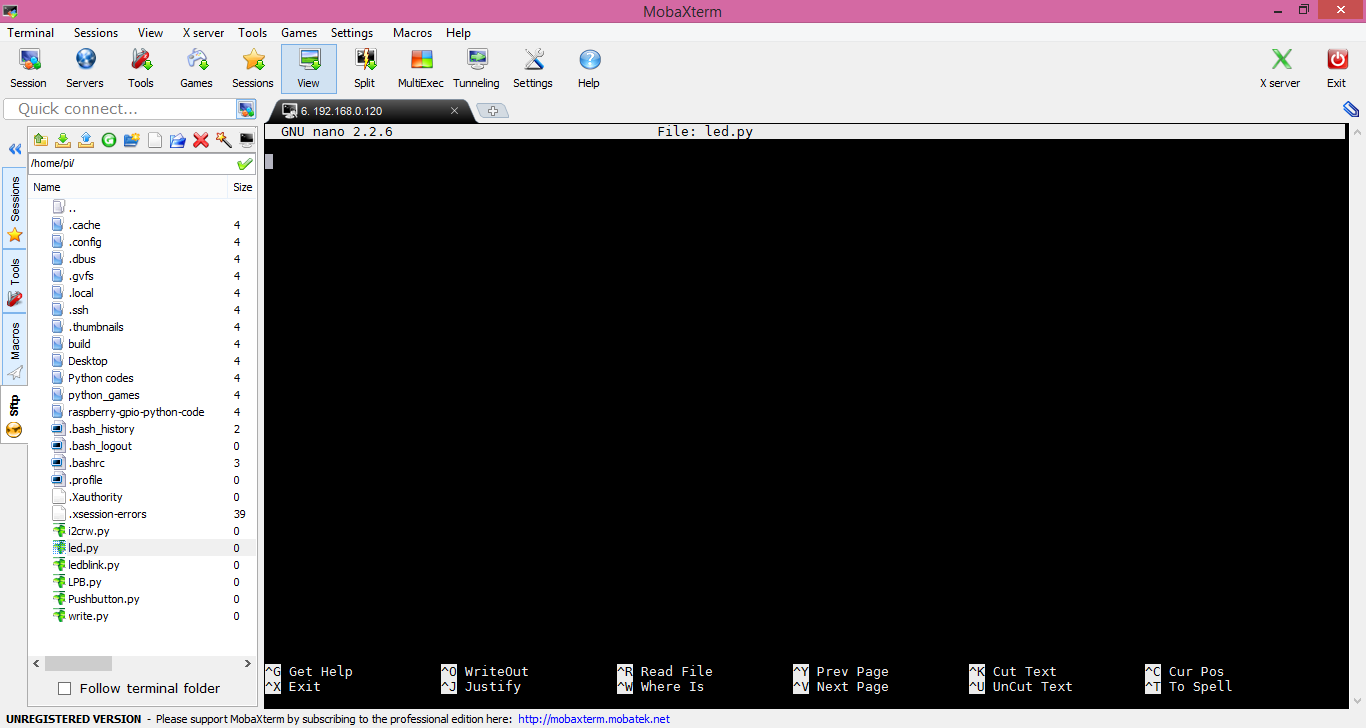
\includegraphics[scale=0.4]{5.png}
					\centering
				\end{figure}
				\item Type the required code and save the contents by typing \textit{Ctrl + X,Y}(to save the file type Y)
				\item Then press enter to exit the editor onto terminal window.
				\item You can now execute the file by using the command \textit{sudo python filename.py}(Don't forget to change the directory if your file is not saved in the home directory.PLease refer the steps mentioned before in the document)
			\end{enumerate}
			Note: Just in case you want to view the contents of the file on the terminal window type \textit{cat filename.py}
		\end{itemize}				
	\end{enumerate}
	\vspace{0.3cm}
	Now we are all set to write basic programs to access GPIO pins in your R-Pi
	
	\newpage
	\section{Experiment}
	 In order to access GPIO pins we need to use the Rpi.GPIO package which is usually present in the Python libraries. (but if you are using an R-Pi 2 please ensure that the version of this package is greater than 0.5.10 )
	 
	 \subsection{Interfacing an LED with R-Pi}
	 \textbf{Setting up the Hardware}
	 \begin{figure}[h!]
	 	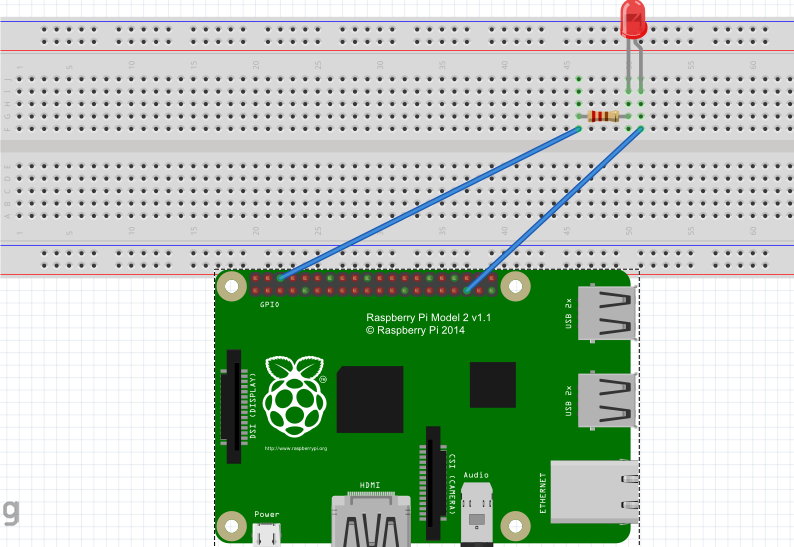
\includegraphics[scale=0.4]{Led.png}
	 	\centering
	 \end{figure}
	 \newline
	 As shown in the figure :
	 \begin{itemize}
	 	\item Anode of the LED is connected to pin no. 18
	 	\item Cathode of the LED is connected to a resistor(330 ohms) which is in turn connected to GND pin on R-Pi 2.
	\end{itemize}
		Note: Please refer the theory section for the pin description of R-Pi 2.
	
	\newpage
	\flushleft
	\textbf{Code}
	\lstinputlisting[language=Python]{ledblink.py}
	
	\newpage
	 \subsection{Interfacing a Push button with R-Pi}
	 \textbf{Setting up Hardware}
	  \begin{figure}[h!]
	  	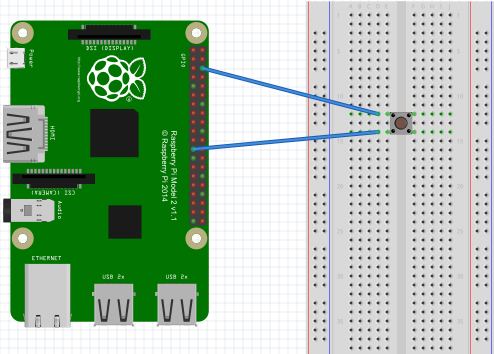
\includegraphics[scale=0.6]{pb.png}
	  	\centering
	  \end{figure}
	   As shown in the figure :
	   \begin{itemize}
	   	\item One pin of the push button is connected to Ground
	   	\item The other pin of the push button is connected to pin no. 12
	   \end{itemize}
	    Note: Please refer the theory section for the pin description of R-Pi 2. Also ensure that the push button pins you connect to R-Pi shoudlnt be shorted.
	    \vspace{0.3cm}
	    \newline
	    \textbf{Code}
	    \lstinputlisting[language=Python]{Pushbutton.py}
	 
	 \newpage  
	\section{Exercise}
	Now that you know how to write simple programs to access GPIO pins of an R-Pi, try your hand at the following problems
	\begin{enumerate}
		\item Controlling an led using a push button. The setup is shown below.
		\begin{figure}[h!]
			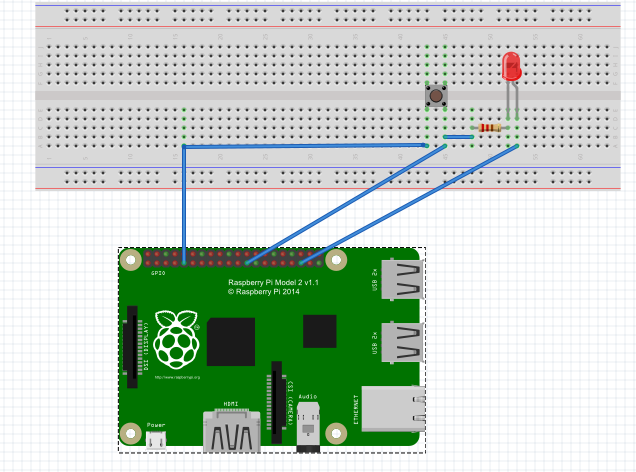
\includegraphics[scale=0.4]{GPIO.png}
			\centering
		\end{figure}
		\item Generating a PWM signal on a GPIO pin to drive an LED 
	\end{enumerate}
	
	\section{References}
	\begin{enumerate}
		\item \url{http://www.engadget.com/2012/09/04/raspberry-pi-getting-started-guide-how-to/}
		\item \url{https://www.raspberrypi.org/products/raspberry-pi-2-model-b/}
		\item \url{http://pi4j.com/images/j8header-photo.png}
		\item \url{http://data.designspark.info/uploads/images/53bc258dc6c0425cb44870b50ab30621}
	\end{enumerate}
	
	
\end{document}



